\documentclass{article}
\usepackage{parskip}
\usepackage{pdfpages}
\usepackage[margin=.6in]{geometry}
\begin{document}

\includepdf[pages=1-3]{slides}
We talked about the ways that life might have occurred on earth. Its very probably that it happened without outside force, which means that it could happen on other planets.


\includepdf[pages=3-6]{slides}
Just remember the shit from astro 101.


\includepdf[pages=7-8]{slides}
The kind of start determines where the habitable zone is, habitable zone is just where liquid water can exist.


\includepdf[pages=9-14]{slides}
Exoplanets are very hard to detect because they only emit reflected light from their sun, but the star is so powerful it hides the planet. We dont really see them, instead we have indirect proof.

The planets subtly alter the stars location due to the effect of gravity and we can see this wobble. The sun should give off perfect light but there are little spots in the atomic spectrum there are tiny particles in the star's atmosphere and we can use these spots to see if the star is red shifted or blue shifted and from this we can see if the star is moving closer or farther from us. This is how we measure the wobble and know how the star is moving. This gives us the mass of the planet. We can use the period of the wobble to know how far the planet from the sun. This will tell us if it is in the habitable zone.


\includepdf[pages=15]{slides}
We can also learn alot about planets that are planar to us.


\includepdf[pages=16]{slides}

\includepdf[pages=17]{slides}
We frequently compare the planet's density to water. We know this because we can get its size and mass. Its crazy what we know.


\includepdf[pages=18]{slides}
The kepler mission was awesome. It brought back a ton of data. For instance this is the orbital time for known planets (we need three sightings for this).11


\includepdf[pages=19]{slides}
Its much easier to see planets that are closer to their star so we have more data on them.

The green band on the second picture shows where liquid water might exist.


\includepdf[pages=20]{slides}

\includepdf[pages=21]{slides}
We recently discovered some very promising planets.

\includepdf[pages=22-27]{slides}

Potential question for assignment = \emph{could life evolve on a water world?}


\includepdf[pages=28-32]{slides}
For life to exist all the laws that we have have to be the same, but these are universal laws so its reasonable.


\includepdf[pages=33-42]{slides}
Life on early basically happened immediately after the late heavy bombardment caused the right conditions. This implies that the transition between chemestry and biology is easier than we think.


\includepdf[pages=43]{slides}
When we looke at the rates of oxygen throughout the history of earth we can see that there have been 5 massive extinctions. Right after these dips we see spikes implying that life comes right back up after the extinction.


\includepdf[pages=44-46]{slides}


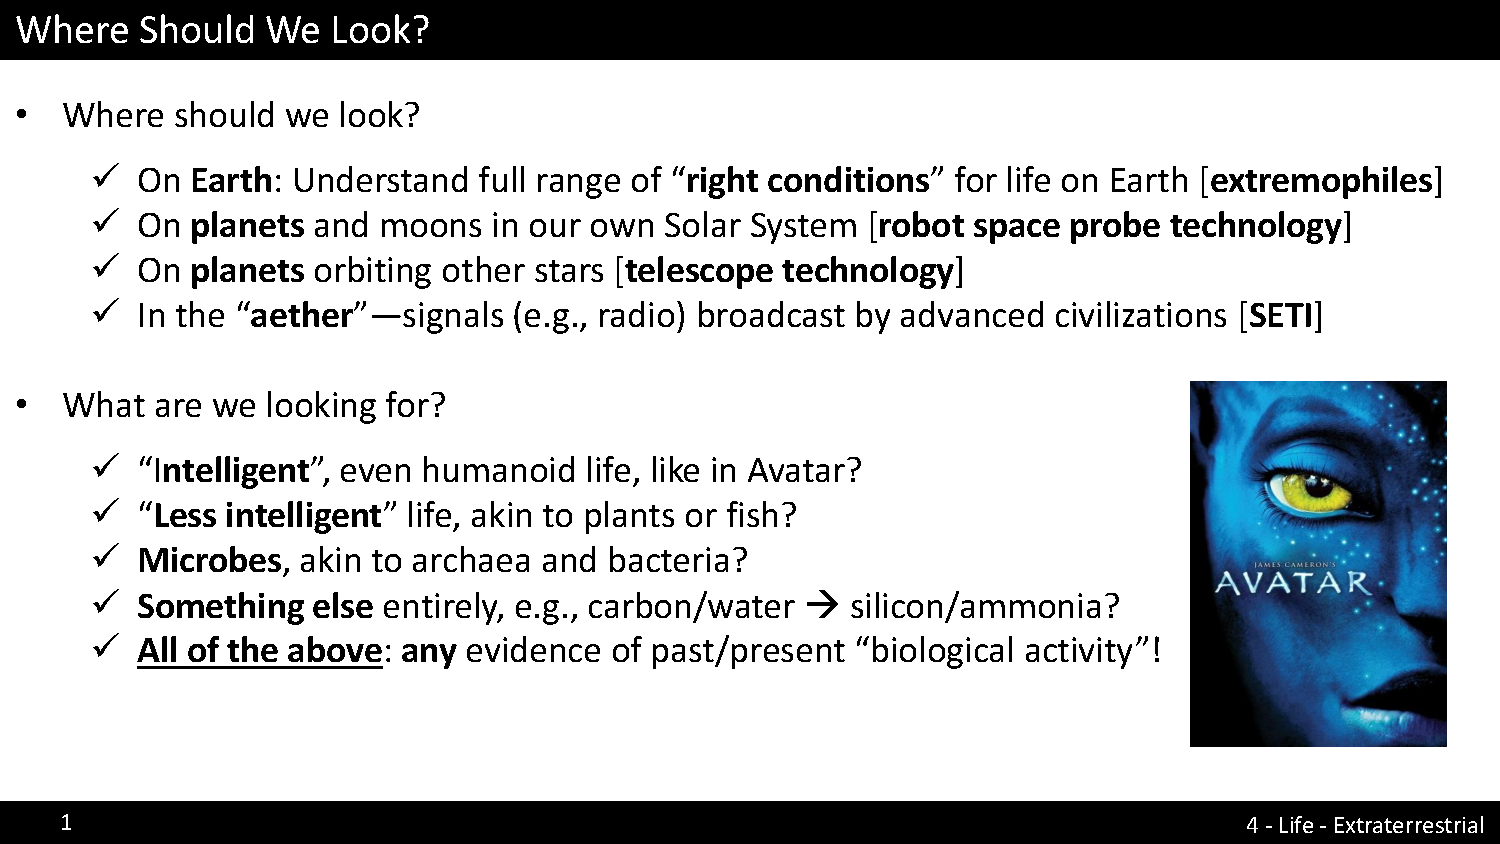
\includepdf[pages=1-2]{slides2}
Its possible that we could have life arrive under different circumstances, using different elements. Life only uses 25/92 of the naturally ocurring elements,

\includepdf[pages=3-4]{slides2}
We need liquid because stuff as to move around to break things down and reform them. They are required for transporting things used in the processes of life. Water in particular is very important because it has many unique properties (is polar for dissolving, made of common elements, is less dense when frozen).

\includepdf[pages=5]{slides2}
If you have life in a cold liquid its metabalism is slower and vice versa.

\includepdf[pages=6]{slides2}
Titan has rocks made out of water and an nitrogen rich atmosphere.

\includepdf[pages=7]{slides2}
One of most important things needed for life is actually just the weird fact that neutrons weigh more than protons. Without this we couldnt really get chemisty rolling. From there we get the molecules neded to build organisms.

\includepdf[pages=8]{slides2}
We need chemestry to build organisms, a source of free energy to fuel metabolism, and finally a liquid medium to move stuff around in. The first two conditions are not all that uncommon, one is a universal rule the other comes from stars, so the main limiting feature is the presence of water. Weirdly enough we also need tidal forces.

\includepdf[pages=9]{slides2}
Without an atmosphere on the moon there is no way to distribute the temperature which causes immense temperature fluctuations during the day. Water also helps even out the heat. The moon does have water, but its frozen on the poles.

\includepdf[pages=10]{slides2}
Believe it or not, life is more likely on venus. It has an atmosphere which actually heats everything up due to how dense the air is. The soviets sent a probe which landed on it and then immidiately melted. There are continents and TONS of volcanoes. There is other evidence of techtonic activity. We known that there was a time of immense technonic shifting which means that any proof of life is surely lost.

\includepdf[pages=11]{slides2}
Venus has a run away greenhouse effect. The two planets are very similiar and had nearly identical starts. The initial atmosphere was formed the same way (volcanoes spewing water vapor). Earth is slightly cooler which allows the water to form clouds and make rain which then makes oceans and the whole water cycle shebang. The water in the atmosphere helps to dissolve C02 out of the atmosphere and rain it down into the ocean. This C02 in the ocean gets seemed into rocks, these rocks then get subducted under the crust and are then spewed into the atmosphere in a C02 cycle.

Venus is much warmer than earth which prevents it from the equilibrium needed for a sustainable cycle. More water evaporated than rained which resulted in the oceans drying up so there was no way to scrub C02 from the atmosphere which causes the run away greenhouse effect. The excessive radiation dissassociates the water into hydrogen and oxygen, the hydrogen escapes and the oxygen reacts with carbon in the rocks to make C02.

\includepdf[pages=12]{slides2}
\includepdf[pages=13]{slides2}
It looks like mars is a bit warmer than earth and started with a slightly thicker atmosphere. It was also fairly wet as well. The planet is slightly smaller than earth which lowered the pressure of the atmosphere which caused water to boil away.

\includepdf[pages=14]{slides2}
Mars is half the diameter of earth, so a quarter of the surface area and one eighth the volume. This means the ratio of surface are to volume is twice that of earth. Remember that planets are full of molten rock. Since its volume is much less it has less internal area but has way more surface area (ratio wise) to give off all the energy it had. This resulted in the end of volcanic energy and the loss of its magnetic field (the center is no longer liquid and thus no longer spinning). This contributed to the loss of the atmosphere because the magnetic field no long deflected the charged particles from the sun. Due to the loss of the atmosphere there is also no ozone layer so the surface gets fucked by UV rays. So unlike venus mars lost all of its greenhouse effects which caused it to be very cold and dry.

\includepdf[pages=15-20]{slides2}
Theres tons of ice at the poles of mars, most of it is water ice but some is carbon dioxide ice. Mars is tilted like earth so it has seasons. So during the summer the carbon dioxide turns into gas, a very large portion actually. So the atmosphere flows from the south pole and causes some real cool dust storms. Theres a fair amount of water that we can see on the surface (enough to cover the planet in 35m of water) and even more underground.

\includepdf[pages=21-26]{slides2}
The immense pressure on these gas giants causes hydrogen to crystallize in a weird latice structure which forms the core.

\includepdf[pages=27]{slides2}
It rains helium droplets which is boss.

\includepdf[pages=28]{slides2}
Life is unlikely. There is no solid ground so if you fell into the planet until you matched the desity of the hydrogen around you. To get hydrogen as dense as water it takes tons of pressure which would make it about as hot as the surface of the sun. Its possible that the right conditions exist, but not statically.

\includepdf[pages=29]{slides2}
Europa gets tidal forces from jupiter which keeps bending the rock around it but this friction warms up the moon. The theory is that this could lead to a liquid ocean.

\includepdf[pages=30]{slides2}
The surface looks solid with a bunch of cracks all over the place but under it there is probably liquid oceans. We currently dont know what kind of ocean it might be. These flowing oceans could create a magnetic field. We know that the water is salty based on the strength of the magenetic field. It is possible that this is enough to support simple life.

\includepdf[pages=31]{slides2}
Titan has a very thick organic rich atmosphere. There is a rocky core and water stuff on top if it. Its under super high pressure so its solid. Due to the extreme cold this surface would be hard as granite.

\includepdf[pages=32-33]{slides2}
Has the thickest atmosphere of the moons in our solar system. Its also very chemically active. In 2013 we landed on the surface. By using radar we can identify where there are liquids (they are perfectly flat and thus reflect a certain way) so we think there might be methane oceans.

\includepdf[pages=34-36]{slides2}
We can learn alot about a planet just from observing the light being emited from it.

\includepdf[pages=37]{slides2}
Life dramatically changes the atmosphere of a planet so we can mimic what earth's atmosphere would be at different times to see how life effected it,

\includepdf[pages=38-42]{slides2}

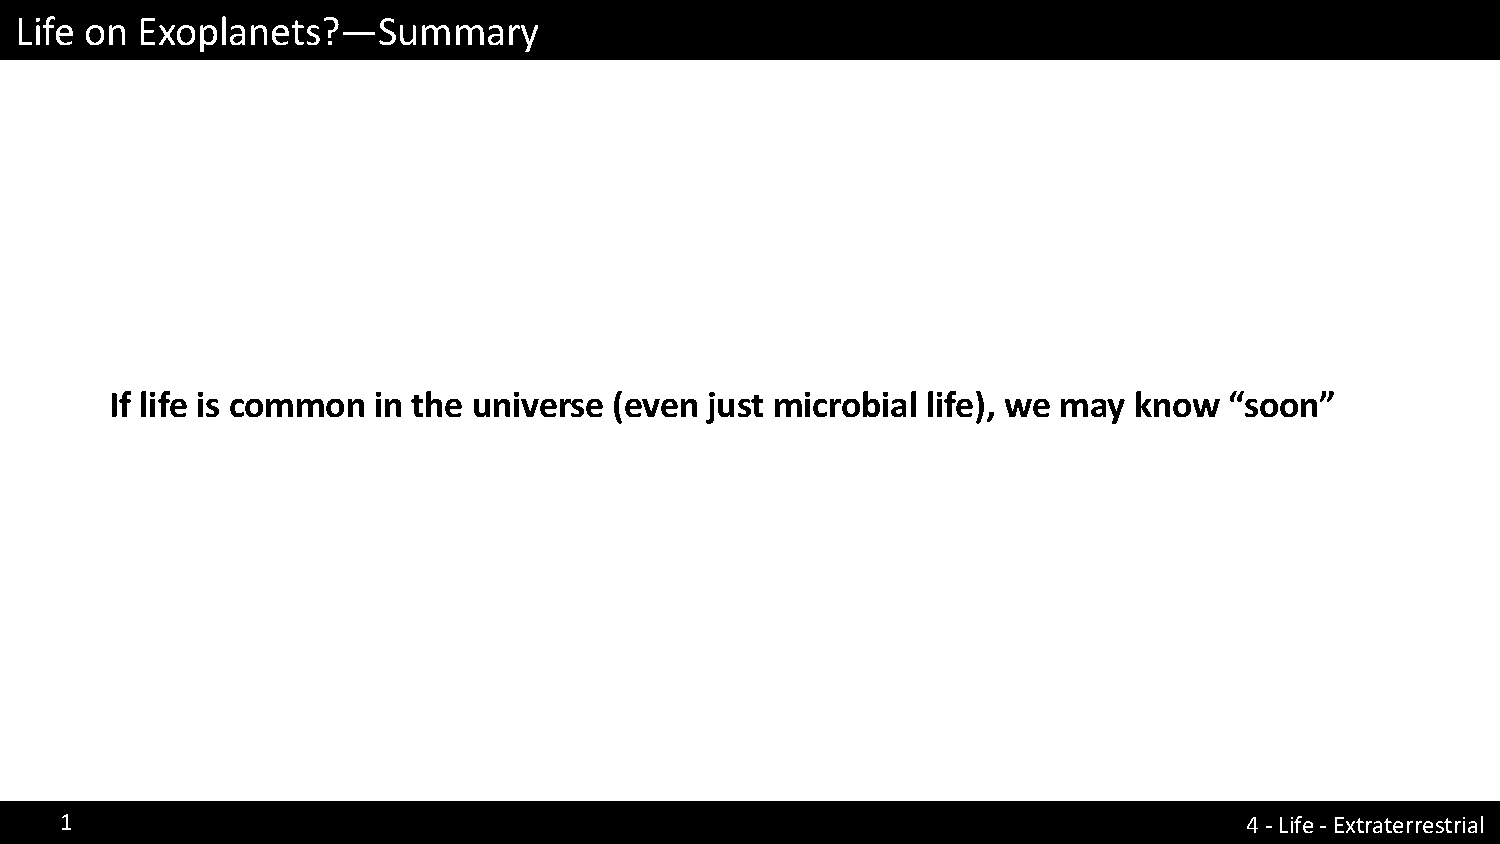
\includepdf[pages=1-2]{slides3}
We are listening really hard to hear when aliens contact us since we are a long way off from us contacting them.

\includepdf[pages=3-8]{slides3}
Everywhere you look there is background radiation and we are looking for anything higher than that. In 1977 they discovered a signal that is 30 times as powerful as the background radiation. They got super excited about this, but its never been repeated and we have no explanation for it.

\includepdf[pages=9]{slides3}
As a response to the wow signal we decided to transmit a signal to the location of it. They sent 10 thousand twitter messages. Not sure why.

\includepdf[pages=10-20]{slides3}
Convergent evolution, when life first emerged it was blind. Eventually the organism needed the ability to sense light and dark. This explodes in complexity into multicellular organisms. Most organisms are able to see. The ability to see has emerged multiple times independently. As our vision becomes more complicated our brains needed to evolve to process it all. Roughly 10\% of our brain is used for this.

\includepdf[pages=21-43]{slides3}

%TODO: FIGURE OUT WHAT SLIDE WE ARE ON, ITS 120 IN THE FULL SET BUT WHO THE FUCK KNOWS
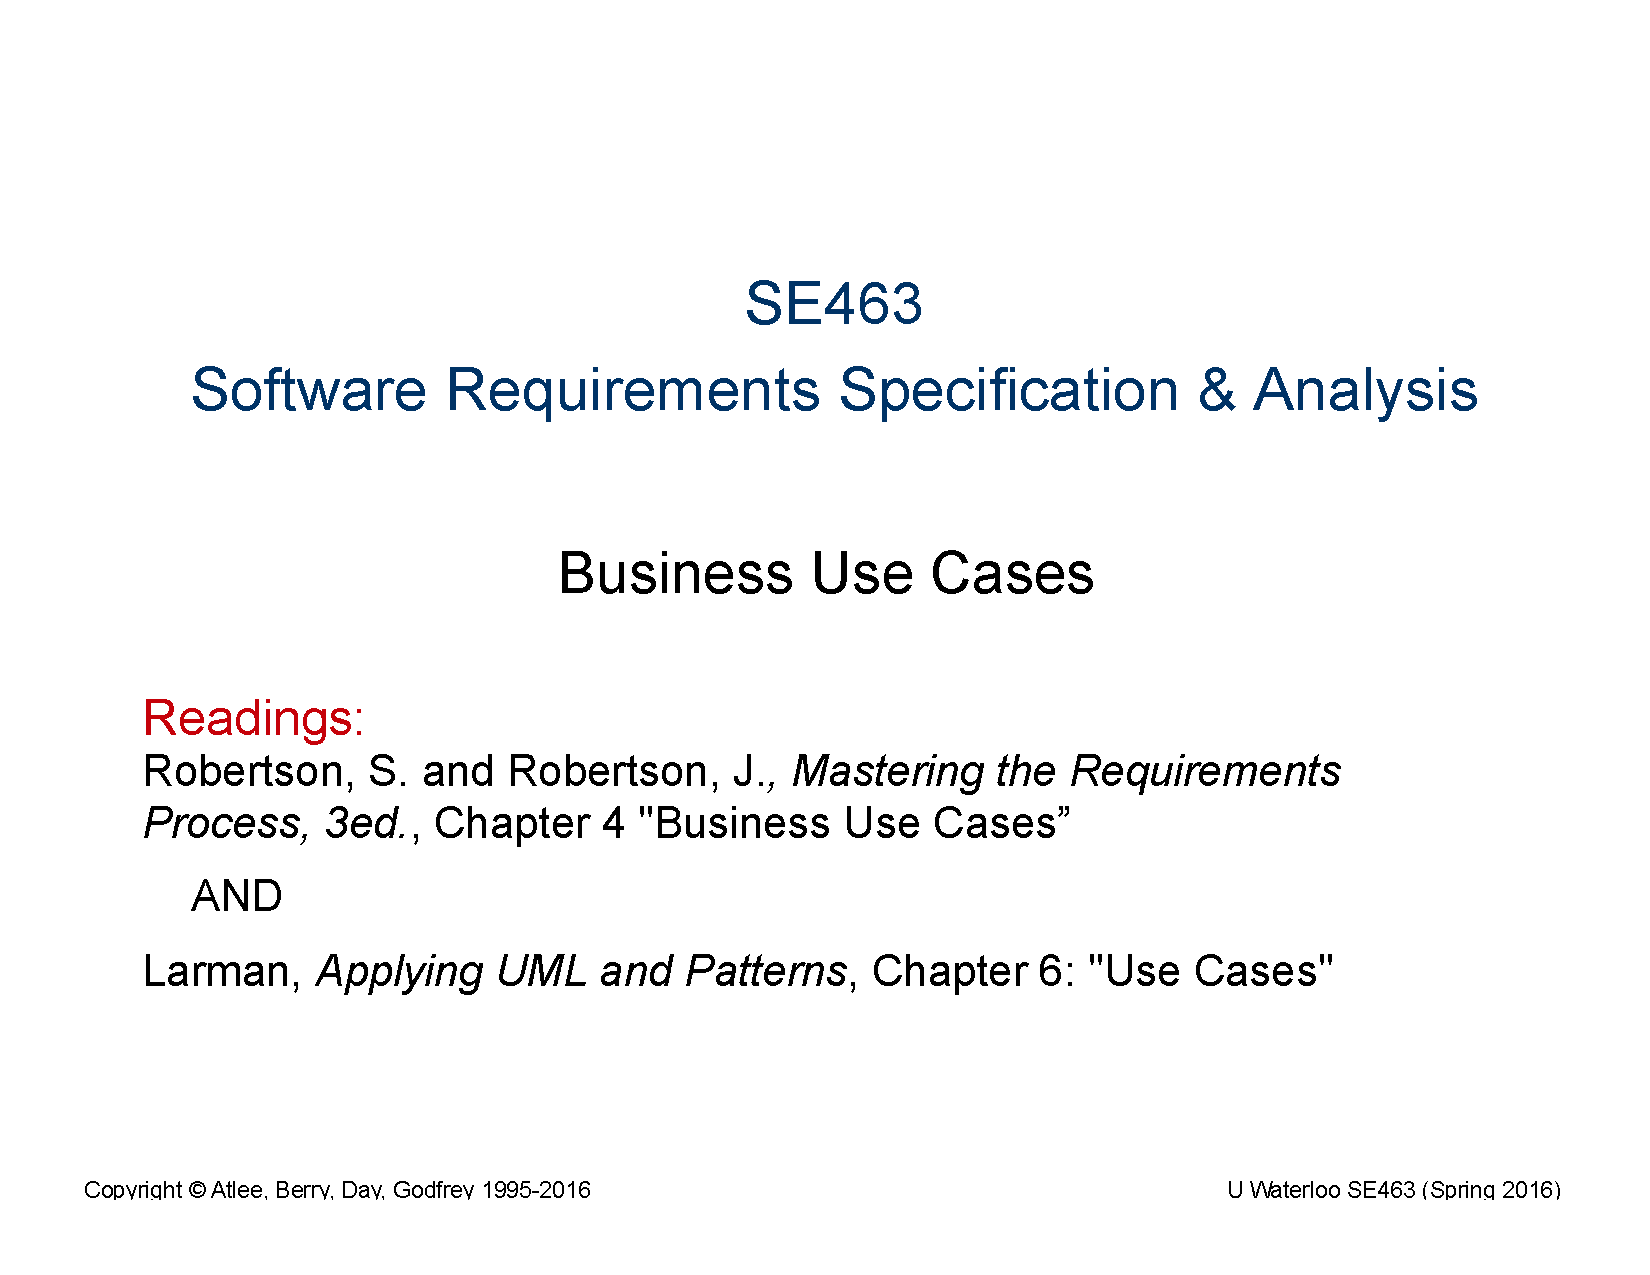
\includepdf[pages=1-]{slides4}
\subsection{Galactic Red Shift}
\label{par:galactic_red_shift}
Galactic red shift shows that galaxies appear to be moving away from us due to the red shift we see. Hubble was the first that noticed this pattern based on his data. It wasn't perfect due to limited tech so we can say more conclusively that he was right. This expansion lets us calculate the age of the universe.

The working models is called the lambda CDM model. We think cold dark matter (CDM) is the majority of the mass in the universe. Lambda is the cosmological constant for dark energy and using this model we estimate the age of the universe as roughly 14 billion years. Its not perfect, but its our best model.

If space is in fact expanding then as we go back in time things should become more dense and hotter. This is how we assume the universe started this way. We have some evidence for this.

\subsection{Cosmic Microwave Background}
\label{par:cosmic_microwave_background}
We have new detectors that can see all wavelengths of light (this is relatively new ability). Microwaves have a soft glow all over the place. This is a huge piece of evidence for the big bang.

The farther out we look into space the farther back in time we see (light has to travel). This allows us to see how galaxies evolve over time. They started out much more irregular in shape and much more dynamic with black holes at the center that did crazy stuff. Galaxies also get denser as we look farther back. There are also many more galaxy collisions. We can see that there are subsets of stars in the milkyway that are moving a specific direction which tells us a collision happened in the past.

How far back can we look? We can look back to within 380 000 years of the big bang which is crazy. There is a veil there that we cannot see past. In every direction the sky is glowing with thermal radiation left over from the big bang. This is almost uniform with small fluctuations (like  1:100 000) of denser matter.
The intensity of light relative to its temperature is not linear. This means that we can measure the intensity of the background radiation and plot it on a curve. It perfectly matches a black body. Its the most perfect black body scientists have ever seen.

About 20 minutes after the big bang all space was filled perfectly uniformly with photons, electrons, and atomic nuclei. At that time there universe was too hot for life to travel properly. This is why we cannot see to the big bang.

When background microwaves were discovered people were confused af. They kept making sure that there was nothing wrong with the telescope. Another guy was trying to prove the existence of the noise that people were seeing and couldn't explain. They asked that guy said they'd been scooped because someone had proved what they were working on before them.

\subsection*{Abundance of Light Elements}
\label{sub:abundance_of_light_elements}
It was too hot to have stable nuclei. Heavier elements kept getting smashed apart. As the universe cooled you could get the lighter elements like helium and hydrogen. To make heavier elements you need a start to do it. There was only a short time (3-20 minutes) during which nuclear fusion could happen. After that you had basically only protons and electrons and maybe some stable hydrogen and helium.

When we ran the math we got that there should be a 7:1 ratio between protons and neutrons. These are all floating around until some fusion happens. So for every helium you need 12 protons. The mass of each helium is equal to a set of four protons. Mass wise you should have roughly 3 times as much hydrogen as helium. So if the big bang happened the universe should have 75\% hydrogen and 25\% helium which we do. EEEYYYY

We can also predict the abundance of other elements. There really isn't much of them but we know how much.

\subsection*{Mystery of Dark Energy}
\label{sub:mystery_of_dark_energy}
We know based on the size of the blobs in the cosmic background radiation that the universe is flat. Which is very helpful.

If there is less than the critical amount of mass pace should be open with a negative curvature, if it was more than the critical mass it would be close. We fall right between these two values. If we distributed mass evenly throughout the universe there should be about 5 hydrogen molecules per cubic meter. When you look there is only 0.2 of visible matter and 1.1 of dark matter. This means we are missing 3.7 missing mass-energy. This is called \emph{dark energy}.

%%page 161

The angular size of the blobs should be roughly one degree in size based on what we see in the observable universe. This calculation relies on the universe being flat. Since we see what we expect, then the universe is flat.

The expansion of the universe is not measured since we have taken measurements throughout history. They expected the universe to be slowing down in its rate of expansion due to all the mass pulling on eachother. It started fast, then slowed down, then about 500 billion years ago it suddently started accelerating.

From this we conclude that dark energy must exist. Dark energy is weird, it exerts negative pressure but had positive density. To have expansion work the way it does it would take 3.7 H/$m^3$. This also fits with how much energy we need for a flat universe.

The cosmological constant is relatively small. If it wasn't this value, all life would be fucked. Too big and the universe would have expanded so fast for anything to form. Too small and it would be too hot to form.

The weird thing is that we need think its density remains constant through out the expansion of the universe. This means that energy has to be created. Thats a no-no.

Our best guess is that dark energy is actually vacuum energy. This is the energy associated with empty space. If we double the amount of space we double the amount of energy. The whole conservation of energy is kinda unknown. We just dont really understand it all that well.

At any place in space there is a probability that some matter and anti matter might spontaneously appear, or some might disappear. On average there is matter and anti matter in space, both of which have positive energy. This does not violate the conservation of energy. There is some energy associated with these quantum fluctuations. These fluctuations can cause negative energy which corresponds to the effect of dark energy.

In a quantum universe a particle in a limited space cannot have 0 energy. They get claustrophobic and start zipping around. This is done via vacuum energy.

\subsubsection*{Quintessence}
\label{ssub:quintessence}
Some people think that dark energy is a dynamic field that pervades all of space uniformly. This is likened to the 5th element from the ancient greeks. We don't really know how this would work. We think that the universe will eventually end in a ``Big Rip'' where the acceleration is too much and the universe just gets ripped apart.

\subsection*{Cosmic Microwave Background}
\label{sub:cosmic_microwave_background}
The little fluctuations are very useful and all life requires it.









\end{document}
